% Generated by scripts/build.py from frk_items.tsv and reference/parts.json.
\documentclass[10pt,letterpaper]{article}
\usepackage[margin=0.45in]{geometry}
\usepackage[T1]{fontenc}
\usepackage{lmodern,graphicx,xcolor,inconsolata,tikz,longtable,booktabs,array}
\usepackage[hidelinks]{hyperref}
\pdfinfoomitdate=1
\pdftrailerid{}
\pagestyle{empty}
\setlength{\parindent}{0pt}
\setlength{\parskip}{5pt}
\setlength{\emergencystretch}{2em}
\renewcommand{\familydefault}{\sfdefault}
% Shared color roles, generated by scripts/build.py.
\definecolor{frkApplication}{HTML}{075985}
\definecolor{frkSupervision}{HTML}{92400E}
\definecolor{frkSecondary}{HTML}{52525B}

\hypersetup{pdftitle={Field Repair Kit: Part Reference},pdfauthor={Team Rubicon}}
\begin{document}
\begin{minipage}[c]{0.83\linewidth}
\begin{minipage}[c]{1.08in}
\includegraphics[width=\linewidth]{../images/team-rubicon-logo.png}\end{minipage}\hspace{0.16in}%
\begin{minipage}[c]{2.8in}{\fontsize{8}{10}\selectfont\color{frkSecondary} FIELD REPAIR KIT --- PART REFERENCE}\end{minipage}\par
{\fontsize{21}{24}\selectfont\bfseries Chain tensioner kit\par}
{\fontsize{18}{21}\selectfont\ttfamily\bfseries \href{https://rduncangt.github.io/frk-management/parts/ma020071002/}{MA02 007 1002}\par}
{\small\color{frkSecondary} Bin \textcolor{black}{\textbf{D1}} \enspace | \enspace \textcolor{black}{\textbf{2}} spares per kit \enspace | \enspace \textcolor{frkSupervision}{\textbf{S2}} supervision}
\end{minipage}\hfill
\begin{minipage}[c]{0.14\linewidth}\centering
\href{https://rduncangt.github.io/frk-management/parts/ma020071002/}{
\includegraphics[width=0.82in]{images/qr.png}}\par
{\scriptsize\color{frkSecondary} Online guide}
\end{minipage}\par\smallskip\hrule\medskip
\noindent\begin{minipage}[c]{0.40\linewidth}\raggedright{\large\bfseries\color{frkApplication} MS 261 --- chain tensioner\par}{\small Includes items 2--8, including tensioner slide \href{https://rduncangt.github.io/frk-management/parts/11256401900/\#ms261-chain-tensioner}{\textcolor{frkApplication}{\mbox{\texttt{1125 640 1900}}}} (item 3).\par
}\smallskip
{\small\textbf{Item 1 \enspace | \enspace Qty listed: 1}}\par
{\footnotesize\color{frkSecondary} MS 261 C-M spare-parts list, 10/02/2023. Drawing p. 15; parts table p. 16.}\par
\end{minipage}\hfill\begin{minipage}[c]{0.57\linewidth}\centering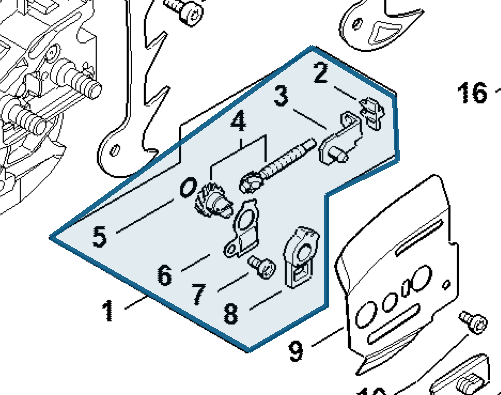
\includegraphics[width=\linewidth,height=3.0in,keepaspectratio]{images/ms261-chain-tensioner.png}\end{minipage}\par\medskip
\noindent\begin{minipage}[c]{0.40\linewidth}\raggedright{\large\bfseries\color{frkApplication} MS 462 --- chain tensioner\par}{\small Includes items 13--19, including tensioner slide \href{https://rduncangt.github.io/frk-management/parts/11256401900/\#ms462-chain-tensioner}{\textcolor{frkApplication}{\mbox{\texttt{1125 640 1900}}}} (item 14).\par
}\smallskip
{\small\textbf{Item 12 \enspace | \enspace Qty listed: 1}}\par
{\footnotesize\color{frkSecondary} MS 462 C-M Z spare-parts list, 10/29/2024. Drawing p. 15; parts table p. 16.}\par
\end{minipage}\hfill\begin{minipage}[c]{0.57\linewidth}\centering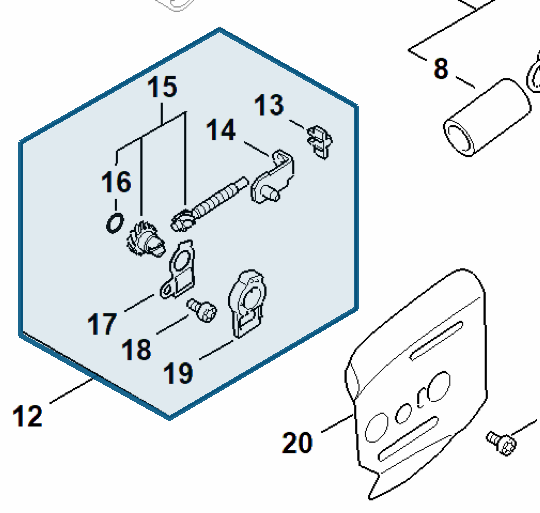
\includegraphics[width=\linewidth,height=3.0in,keepaspectratio]{images/ms462-chain-tensioner.png}\end{minipage}\par\medskip
\vfill\hrule\smallskip{\footnotesize\color{frkSecondary} Drawing \textcopyright{} ANDREAS STIHL AG \& Co. KG. Not to scale.\hfill 2026-09-27}
\end{document}
